\section{Attributes of Dependability}
The attributes specified in \cref{fig:sub_depend} are further defined, as shown in \cref{tbl:rts_depend_crit}.

\begin{table}[ht]
  \centering
  \begin{tabular}{|l|r|}
  \hline
    \textbf{Availability} & Readiness for correct service \\ \hline
    \textbf{Reliability} & Continuity of correct service \\ \hline
    \textbf{Safety} & Absence of catastrophic consequences on the user(s) \\ & and the environment \\ \hline
    \textbf{Integrity} & Absence of improper system alterations \\ \hline
    \textbf{Maintainability} & Ability to undergo modifications and repairs \\ \hline
    \textbf{Confidentiality} & Absence of unauthorised disclosure of informations \\ \hline
  \end{tabular}
  \caption{Attributes of dependability\cite{rts_depend}}
  \label{tbl:rts_depend_crit}
\end{table}

If a system is to be declared dependable, it is necessary to analyse it in the given context in order to provide a weighting of the attributes.
This should be done to determine which attributes are desirable for the given system, and what is irrelevant in the given context.
The weighting then provides a set of criteria for the measures that should be undertaken to ensure dependability.\\
However, these criteria not only apply to a single component, but rather applies to the broader system definition which encompasses all interacting components.
This means that if the criteria are to be applied to a single component, the same criteria will have to be applied to all dependent components.
Alternatively the single component will have to include provisions against failures in dependent components, which ensures that the criteria continues to be met.
The latter will be impossible to achieve in situations where a strong dependency exists i.e. the output of the dependent components is directly transformed into the output of the single component.
In such a case there is no choice but to provision all components in unison if dependability is to be achieved, as the single component has no redundant input source.

\subsection{Attributes of Security}
In relation to security, the interpretation of attributes changes slightly.
Security is defined by the combination of "availability for authorized actions only", "confidentiality" and "integrity with 'improper' meaning 'unauthorized' " i.e. "Absence of unauthorised system alterations".\autocite{rts_depend}

\section{Threats to Dependability}
As shown in \cref{fig:sub_depend}, creating a dependable system also requires that possible threats are analysed and identified, as these dictate the means necessary to maintain dependability. \\
In order to properly define the threats, \textcite{rts_depend} introduces and defines three concepts,
as well as a relationship between these, and the lifetime of a threat, as shown in \cref{fig:rts_threat_life}.

\begin{figure}[ht]
  \centering
  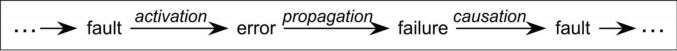
\includegraphics[width=0.8\textwidth]{graphics/depend3.png}
  \caption{Life-time of a threat\autocite{rts_depend}}
  \label{fig:rts_threat_life}
\end{figure}

\subsection{Faults}
Faults are defined as the cause of an error, without limiting a fault to only be the cause of a single error.
A fault may cause multiple errors and a fault may be both internal or external to the system.
In the case of an external fault, an internal fault enables the external fault to cause an error in the system, in this sense the fault serves as a vulnerability, rather than the direct cause of an error.\\
A fault can exists in two possible states, active and dormant, the transition from dormant to active, the activation, happens when a fault causes an error in the system state.

Faults can be introduced during both the development and the use phase of the software, with differing environments capable of introducing different types of faults.
These environments are described in detail in \autocite[14]{rts_depend} and will not be further discussed here.\\
\textcite{rts_depend} introduces 16 elemental fault classes to describe the different fault types.
These elemental fault classes are combined to form, what the authors deem, the 31 combined fault classes likely to be relevant for a dependable system.
Rather than introduce all 31 combined fault classes, the fault classes relevant for the system will be presented during the analysis.

\subsection{Errors}
An error is defined as the part of the total system-state which may lead to the systems subsequent failure.\autocite{rts_depend}
An error need not cause a system failure, however a fault will still have been activated to cause the error.
Whether or not the error manifests as a failure may be accidental or means may have been put into place 
which prevent the error from reaching the external state of system.\\
Different means exist which may be provisioned to make the system more resilient, these will be presented in \cref{sec:depend_attain_depend}.

\subsection{Failures}
A failure, or sometimes service failure, is when the delivered service deviates from correct service.\\
This deviation can take multiple forms and range from a total system failure to a partial failure and reduction in service delivery.
This naturally leads to the definition of multiple failure types, of which \textcite{rts_depend} distinguish between many,
but also leads to the classification of the failure types with regards to severity, in terms of the system being analysed.
These failure types are numerous and therefore only the relevant ones will be brought up in the analysis.
For a full definition of the different failure types, see \autocite[18-20]{rts_depend}.

\section{Means to Attain Dependability}\label{sec:depend_attain_depend}
Four means of attaining dependability are specified and defined; fault prevention, fault tolerance, fault removal and fault forecasting.
These methods all serve to provide and increase dependability, but they differ vastly in their approach.\\
Fault prevention, and fault removal during the use phase are similar in that both means focus on the development task in order to attain their goal.
Fault prevention is concerned with initial development and fault removal during use is concerned with the maintenance task.
These two means are very process-centric and focus on improving the development process to minimise the number of faults being introduced.\\
Fault removal during development focuses on attaining the goal by analysing the system.
Fault removal employs various analysis or modelling and model verification techniques, to attempt to detect and remove faults before the system enters the use phase.\\
Fault forecasting differ from the other means in that it is not a means of preventing the occurrence of failures,
rather it is a means of measuring the dependability of the system.\\
Fault tolerance is the method which is of the greatest interest for our system.
It differs vastly from fault prevention and fault removal in that it does not seek to eliminate faults,
but rather accepts that faults will be introduced and errors will occur,
and seeks to make the system dependable by detecting these errors and recovering from them before they become failures.

\section{Dependability of Our System}

In this section our system, as specified in \cref{sec:base_setup}, will be analysed in its context with respect to attributes and threats affecting the dependability of the system.
The system will be analysed as a whole rather than subdivided into individual components.
This means that failures occur when errors are visible outside the system, and an internal failure between components is not a system failure.
Likewise this affects the user(s) of the system as these become the people and external systems who rely on the system for surveillance, tracking and potential intervention.
Means to attain these attributes and to handle these threats will then be described and provisions for ensuring dependability will be defined.\\

\subsection{Attributes of Our system}
Each of the 6 defined attributes will be examined in turn and if an attribute is deemed relevant, its importance is assessed.\

\subsubsection{Availability \& Reliability}
Availability and reliability are defined as the readiness of respectively the continuity of correct service.\\
These attributes are both very important as the systems primary task is to provide surveillance and tracking.
This necessitates that the system be available for service at any time.
This makes reliability important, as frequent service outages will result in low availability in use environments 
where operators are infrequently available and where operator coverage is low in general.

As such availability and reliability both have a high priority for the dependability of the system

\subsubsection{Safety}
Safety is defined as the absence of catastrophic consequences on the user(s) and the use environment.\\
For the system's primary task of surveillance and tracking, safety is an unimportant attribute for dependability.
In the system's primary task it is essentially passive, only recording and relaying information.
System users who rely on this information may have Safety as an important attribute but this will not affect the system.\\
However safety may become important with introduction of the system's secondary task of intervention.
If the nature of the intervention is such that it has the capability to inflict catastrophic consequences,
safety should be a consideration when configuring the system for use.

Safety is deemed an unimportant attribute for the design of the general system.
Depending on the individual configured system, it should however be taken into account.

\subsubsection{Integrity}
Integrity is defined as the absence of improper system alterations, or in the context of security, as the absence of unauthorised system alterations.\\
As the information gathered and provided by the system is likely vital for the systems intended use, integrity is a very important attribute of the dependability of the system.
If the system provides a way of remotely modifying or altering the system, the definition with respect to security becomes highly relevant as well.
This importance is further stressed if the system's secondary task of intervention is taken into account.

Due to the nature of the information gathered it is paramount that the system be trustworthy.
This makes integrity more important than availability and reliability, as those two attributes become irrelevant if the system cannot be trusted.

\subsubsection{Maintainability}
Maintainability is defined as the ability to undergo modifications and repairs.\\
Due to system's intended use it is all but expected that malicious attempts at damaging the system will happen.
Because of this it is important that the system be maintainable to allow quick facilitation of modifications and repairs to mitigate these attempts.

Despite maintainability being important it is deemed as less important than availability, reliability and integrity.
The reasoning behind this assessment is that attempts to damage the system is unlikely to be the easiest way to disable the system unless a high level integrity is provisioned.
Likewise if the system has poor availability and reliability it may be unnecessary to disable the system as frequent breakdowns will serve any need to avoid the system.

\subsubsection{Confidentiality}
Confidentiality is defined as the absence of unauthorised disclosure of information.\\
In spite of the vital nature of the information gathered and internally and externally by the system it is not sensitive in nature.
While an unauthorised disclosure of information is likely to affect the trustworthiness of the system, 
the system need not provision to avoid this as the integrity is not affected.

Confidentiality is deemed a relevant attribute of the dependability of the system due to its effect on the trust put into the system.
However it has the lowest priority of the relevant attributes and will likely be disregarded in the design and viewed as an auxiliary, non-functional feature.

\subsubsection{Weighting of Attributes}
Availability, reliability and integrity are all deemed very important for the dependability of the system, with integrity being paramount for it.
Maintainability and confidentiality are both deemed less important attributes and should only be provisioned for if it can be done without negatively affecting the more important attributes.

\subsection{Threats \& Provisions}
This section presents the discovered threats to our system and the provisions which can be employed to increase dependability of the system.
The list is not claimed to be exhaustive based on the generally accepted notion that ''there will always be faults present'',
it is likely that further analysis will add more items to the list.\\
However the section will present the most prominent threats and the provisions against them.

\subsubsection{Erroneus object recognition}
A very prominent fault stems from the use of pattern matching algorithms.\\
The information provided by \gls{opencv} is obtained using an algorithm which provides a 'best match'.
Because of this there is a risk that camera units recognise the wrong object and thus incorrect information is disseminated to the rest of the system.\\
As this fault is due to a technical limitation it does not fit neatly into the elemental fault classes defined by \textcite{rts_depend}.
For the determination of intent it is neither a deliberate fault nor is it a non-deliberate fault, it is merely a limitation.
Because of this no attempt to fit the fault into the elementary categories will be made.

To provision against this fault, fault tolerance can be employed in three locations.\\
The first location where the information is obtained, a threshold value for the match probability can be set.
If the probability falls below this lower bound, the information will be discarded as erroneous and provide no information.\\
The second location utilises the presence of an surplus of data.
If the difference in information from a single camera unit exceeds a threshold value,
the information is considered erroneous and will not be used for the tracking calculations.\\
The third location requires the definition of a maximum achievable velocity of an object.
If the maximum velocity is exceeded by a set of information an error is detected.
If there is an over-abundance of information different subsets of the information can be calculated and checked for a better match, eliminating the singular fault.
If there is only sufficient data to perform calculations this method can merely be used to detect the error but not prevent a failure.

\subsubsection{Lack of information}
A possible threat to the system is the lack of sufficient information.\\
If the system has insufficient information available to perform tracking computations, it has no way to recover and prevent the manifestation of a failure.
This situation is something which must be handled upon configuration of the physical system.
The physical layout of the system has to be designed in such a way that sufficient information is sufficiently likely to be available.\\
The design should allow for zero or more internal service outages among the camera units dependent of what kind of redundancy and dependable is required of the system.

\subsubsection{Disruption of communication}
The presented design uses a wired network which already serves to make the system very resilient against disruption.
In spite of this, disruption can still happen if access to the wired network is achieved and likewise denial of service can be performed.

This fault falls into the category of interaction faults.\autocite{rts_depend}
To provision against this fault the network should be isolated and completely separate,
this will necessitate physical access to the system which, if attained, becomes very difficult to provision against.

\subsubsection{Impersonation}
As integrity is paramount to the dependability of the system, provisions against impersonation and subsequent dissemination of malicious data must be taken.\\
A natural way of provisioning against impersonation will be to implement encryption between all endpoints.
This should be implemented in a way such that a breach in integrity of any component does not result in a breach of integrity for the entire system.
Employing this provision has the added benefit of also providing a means of achieving confidentiality.

\section{Effects on Dependability}
The attributes specifying the criteria for making the system dependable have been selected and weighted according to their importance.
Ensuring a high compliance with these criteria will result in a dependable system.
This compliance must partly be realised by considering the criteria when iterating on the design of the system,
and partly by implementing the defined provisions against the discovered faults.
If an even more dependable system is wanted, this analysis should be repeated and continued with respect to identifying more faults
and provisions against these and the errors they cause.